

\documentclass[a4paper,11pt]{article} 

% ===== Algunos paquetes a ser usados =====

% para poder escribir con tildes
\usepackage[T1]{fontenc}
\usepackage[utf8]{inputenc}
\usepackage[spanish]{babel}

% fuentes para escribir símbolos
\usepackage{amsfonts}
\usepackage{amssymb}
\usepackage{amsthm}
\usepackage{mathrsfs}
\usepackage{hyperref}
\usepackage{graphicx} 


% ===== Encabezado =====
\pagestyle{myheadings}
\markright{Informe Fabian Cordovez Daniel Leiva  Victoria Muñoz \hfill Ingeniera en Software \hfill}
% ======================


% ========  Aca comienza el cuerpo del texto ==========

\title{Metodologías de Desarrollo de Software}
\author{Universidad Tecnológica Metropolitana\\ Facultad de Ingeniería\\
Ingeniera en Software}

\begin{document}

% hace título
\maketitle
%hace índice

\newpage

\section{Metodología Agil}
\subsection{Programación Extrema (XP)}
Es el más destacado de los procesos ágiles de desarrollo de software. Se puede considerar la programación extrema como la adopción de las mejores metodologías de desarrollo de acuerdo a lo que se pretende llevar a cabo con el proyecto, y aplicarlo de manera dinámica durante el ciclo de vida del software.\\
La simplicidad es la base de la programación extrema. Se simplifica el diseño para agilizar el desarrollo y facilitar el mantenimiento. \\
Aplicando la simplicidad junto con la autoría colectiva del código y la programación por parejas se asegura que cuanto más grande se haga el proyecto, todo el equipo conocerá más y mejor el sistema completo.\\
La comunicación se realiza de diferentes formas. El código autodocumentado es más fiable que los comentarios ya que éstos últimos pronto quedan desfasados con el código a medida que es modificado. Debe comentarse sólo aquello que no va a variar, por ejemplo el objetivo de una clase o la funcionalidad de un método.\\
Las pruebas unitarias son otra forma de comunicación ya que describen el diseño de las clases y los métodos al mostrar. La comunicación con el cliente es fluida ya que el cliente forma parte del equipo de desarrollo. El cliente decide qué características tienen prioridad y siempre debe estar disponible para solucionar dudas.\\
Al realizarse ciclos muy cortos tras los cuales se muestran resultados, se minimiza el tener que rehacer partes que no cumplen con los requisitos y ayuda a los programadores a centrarse en lo que es más importante.\\
Muchas de las prácticas implican valentía. Una de ellas es siempre diseñar y programar para hoy y no para mañana. Esto es un esfuerzo para evitar empantanarse en el diseño y requerir demasiado tiempo y trabajo para implementar el resto del proyecto. Esto significa revisar el sistema existente y modificarlo si con ello los cambios futuros se implementaran mas fácilmente.\\
El respeto se manifiesta de varias formas. Los miembros del equipo se respetan los unos a otros, porque los programadores no pueden realizar cambios que hacen que las pruebas existentes fallen o que demore el trabajo de sus compañeros. Los miembros respetan su trabajo porque siempre están luchando por la alta calidad en el producto y buscando el diseño óptimo o más eficiente para la solución a través de la refactorización del código. Los miembros del equipo respetan el trabajo del resto no haciendo menos a otros, una mejor autoestima en el equipo eleva su ritmo de producción.

\newpage
\section{Metodología Tradicional}
\subsection{Proceso Unificado de Rational (RUP)}
El RUP es un conjunto de metodologías adaptables al contexto y necesidades de cada organización.Un proceso de desarrollo de software creado por la empresa Rational Software, actualmente propiedad de IBM. Constituye la metodología estándar más utilizada para el análisis, diseño, implementación y documentación de sistemas orientados a objetos.\\
El RUP está basado en 6 principios clave que son los siguientes:
\begin{enumerate}
\item Adaptar el proceso: El proceso deberá adaptarse a las necesidades del cliente. Las características propias del proyecto, el tamaño del mismo, así como su tipo o las regulaciones que lo condicionen, influirán en su diseño específico. También se deberá tener en cuenta el alcance del proyecto en un área subnormal.
\item  Equilibrar prioridades: Los requisitos de los diversos participantes pueden ser diferentes, contradictorios o disputarse recursos limitados. Debe encontrarse un equilibrio que satisfaga los deseos de todos. La idea es corregir desacuerdos que surjan en el futuro.
\item Demostrar valor iterativamente: Los proyectos se entregan, aunque sea de un modo interno, en etapas iteradas. En cada iteración se analiza la opinión de los inversores, la estabilidad y calidad del producto, y se refina la dirección del proyecto así como también los riesgos involucrados.
\item Colaboración entre equipos: El desarrollo de software no lo hace una única persona sino múltiples equipos. Debe haber una comunicación fluida para coordinar requisitos, desarrollo, evaluaciones, planes, resultados, etc.
\item Elevar el nivel de abstracción: Este principio dominante motiva el uso de conceptos reutilizables tales como patrón del software, lenguajes 4GL o marcos de referencia (frameworks) por nombrar algunos. Esto evita que se vaya directamente de los requisitos a la codificación de software a la medida del cliente, sin saber con certeza qué codificar para satisfacer de la mejor manera los requisitos y sin comenzar desde un principio pensando en la reutilización del código. Un alto nivel de abstracción también permite discusiones sobre diversos niveles y soluciones arquitectónicas.
\item Enfocarse en la calidad: El control de calidad no debe realizarse al final de cada iteración, sino en todos los aspectos de la producción. El aseguramiento de la calidad forma parte del proceso de desarrollo y no de un grupo independiente.
\end{enumerate}

\newpage

\section{Cuadro Comparativo }
\subsection{XP vs RUP}
\vspace{1cm}

    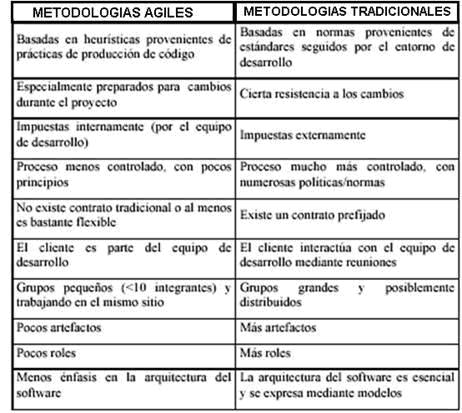
\includegraphics{comparativo}
\newpage
 
\section{Anexo }

Link de Repositorio Github
\begin{enumerate}
\item \url{https://github.com/victoriaMB/Metodologias_De_Desarrollo}
\end{enumerate}

\end{document}
